\begin{figure}[h!]
    \centering
    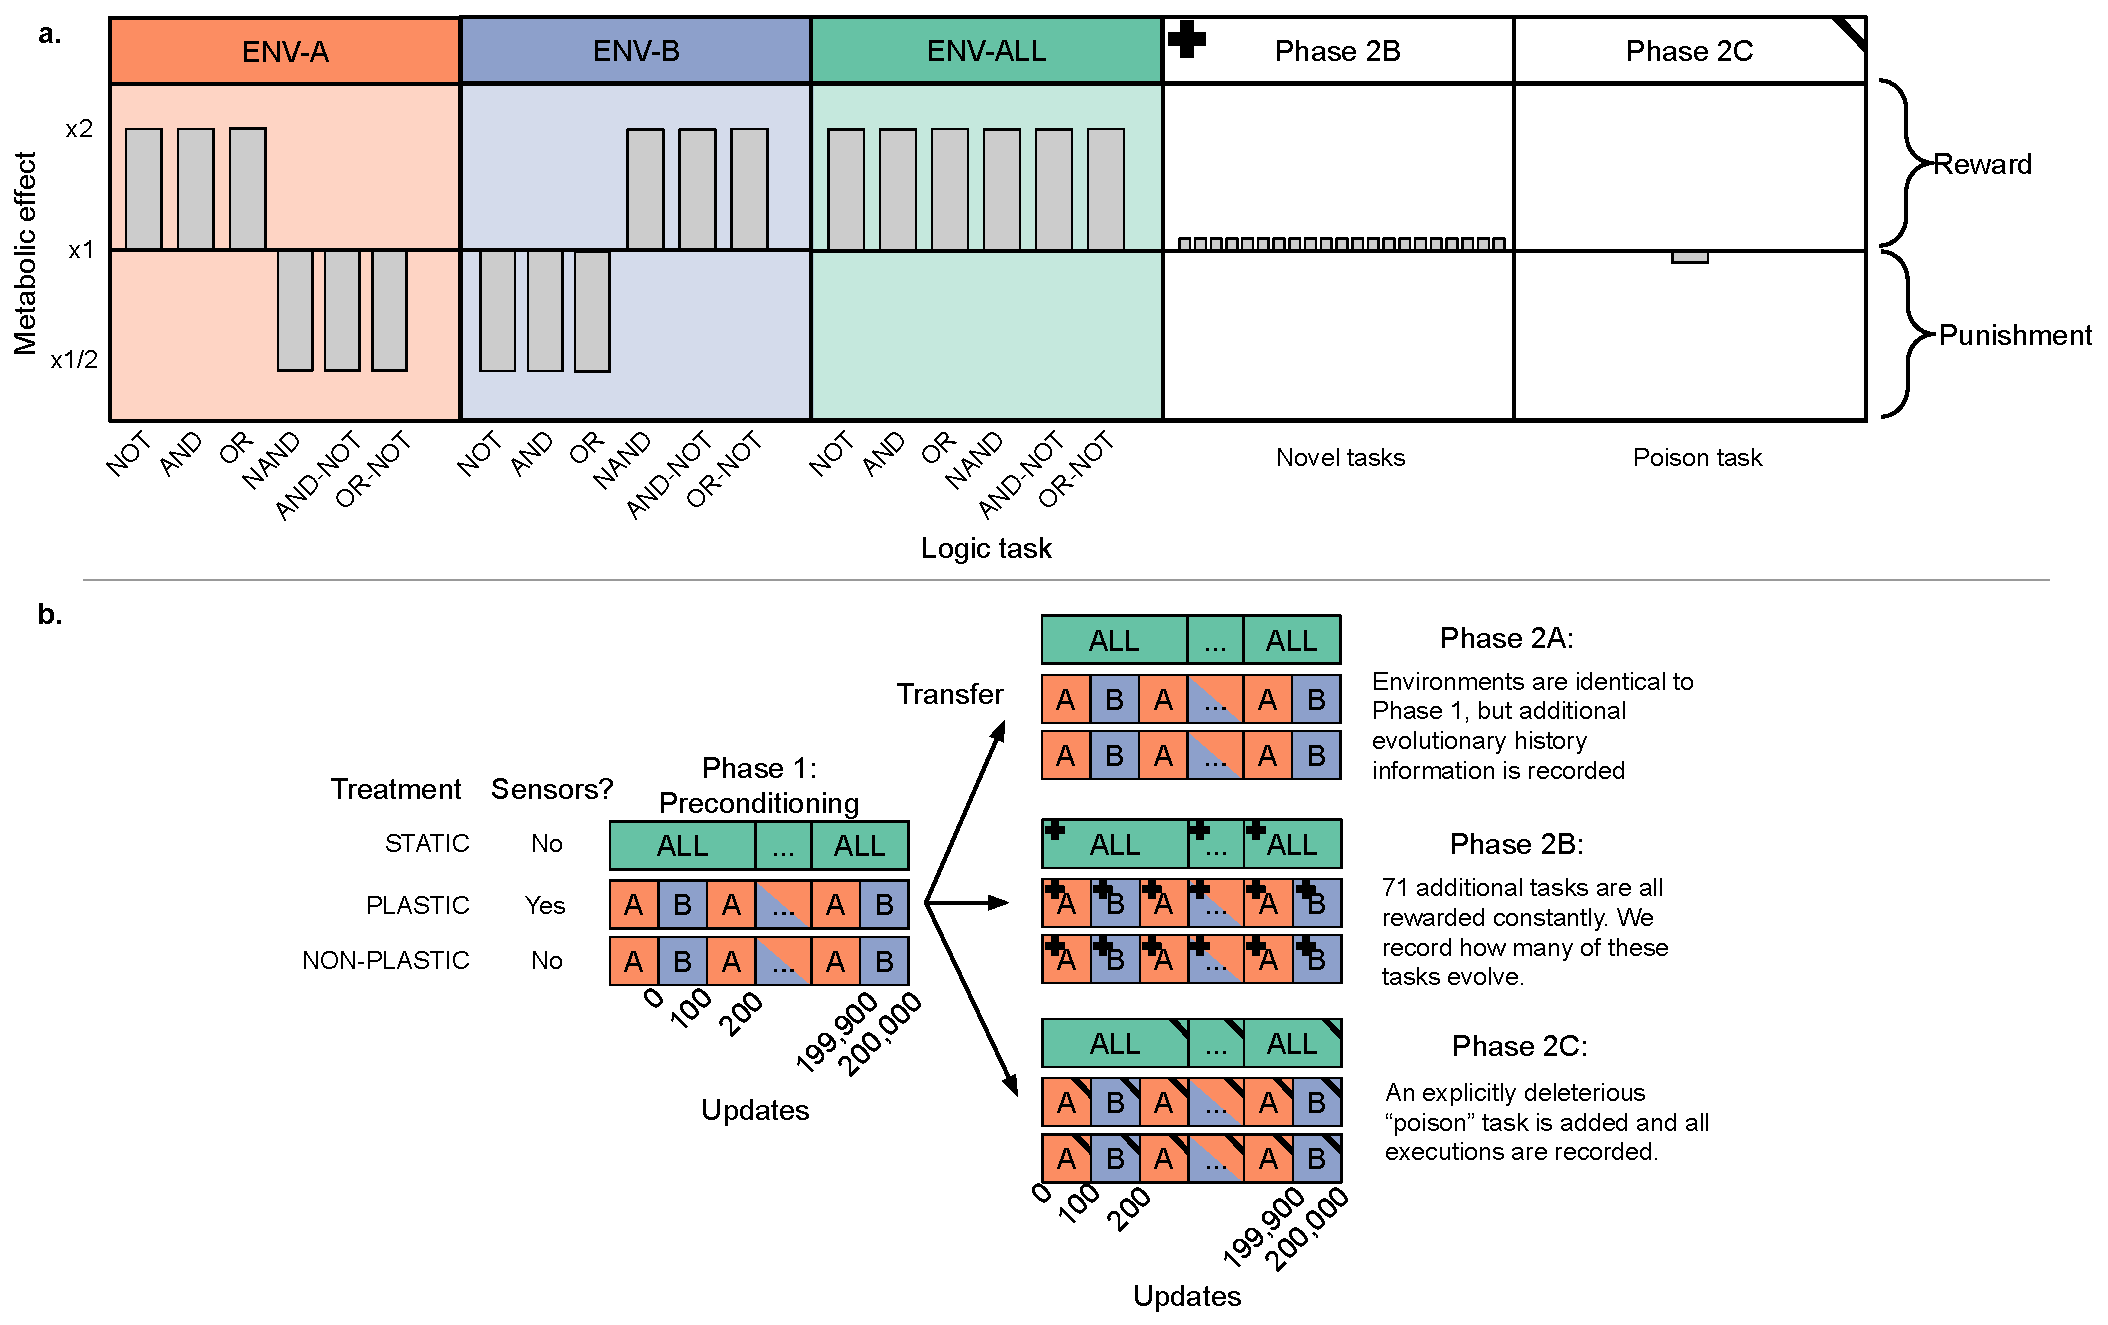
\includegraphics[width=1\textwidth]{media/experimental-design.pdf}
    \caption{\small
    \textbf{Overview of experimental design.}
    Panel a shows the three environments used in every experiment and whether they reward or punish each base task. 
    Additionally, the last two subplots in (a) show the additional tasks added in Phases 2B and 2C. 
    All novel tasks confer a 10\% metabolic reward, while executing the \code{poison} task causes a 10\% metabolic punishment. 
    Panel b shows how treatments are defined and the phase transition. 
    Treatments are defined on the left, with each treatment consisting of an environment timeline and whether sensors are functional. 
    This also shows Phase 1, the preconditioning phase.  
    We conducted experiments using three different second phases, as shown on the right. 
    Phase 1 is repeated for \textit{each} Phase 2, with 100 populations of each treatment. 
    All STATIC and NONPLASTIC replicates move on to Phase 2, while PLASTIC populations are only continued if their most abundant genotype exhibits optimal plasticity. 
    Metrics are recorded only in Phase 2. 
    }
    \label{fig:experimental-design}
\end{figure}